% --------------------------------------------------------------
% This is all preamble stuff that you don't have to worry about.
% Head down to where it says "Start here"
% --------------------------------------------------------------
 
\documentclass[12pt]{article}
 
\usepackage[margin=1in]{geometry} 
\usepackage{amsmath,amsthm,amssymb,dsfont}
\usepackage{graphicx} %package to manage images
\graphicspath{ {./} }
%packages to insert code
\usepackage[svgnames]{xcolor}
\usepackage{listings}

\lstset{language=R,
    backgroundcolor=\color{OldLace},
    basicstyle=\small\ttfamily,
    stringstyle=\color{DarkGreen},
    otherkeywords={0,1,2,3,4,5,6,7,8,9},
    morekeywords={TRUE,FALSE},
    deletekeywords={data,frame,length,as,character},
    keywordstyle=\color{blue},
    commentstyle=\color{DarkGreen},
}

\newenvironment{theorem}[2][Theorem]{\begin{trivlist}
\item[\hskip \labelsep {\bfseries #1}\hskip \labelsep {\bfseries #2.}]}{\end{trivlist}}
\newenvironment{lemma}[2][Lemma]{\begin{trivlist}
\item[\hskip \labelsep {\bfseries #1}\hskip \labelsep {\bfseries #2.}]}{\end{trivlist}}
\newenvironment{exercise}[2][Exercise]{\begin{trivlist}
\item[\hskip \labelsep {\bfseries #1}\hskip \labelsep {\bfseries #2.}]}{\end{trivlist}}
\newenvironment{reflection}[2][Reflection]{\begin{trivlist}
\item[\hskip \labelsep {\bfseries #1}\hskip \labelsep {\bfseries #2.}]}{\end{trivlist}}
\newenvironment{proposition}[2][Proposition]{\begin{trivlist}
\item[\hskip \labelsep {\bfseries #1}\hskip \labelsep {\bfseries #2.}]}{\end{trivlist}}
\newenvironment{corollary}[2][Corollary]{\begin{trivlist}
\item[\hskip \labelsep {\bfseries #1}\hskip \labelsep {\bfseries #2.}]}{\end{trivlist}}
% Created
\newenvironment{solution}[2][Solution]{\begin{trivlist}
\item[\hskip \labelsep {\bfseries #1}\hskip \labelsep {\bfseries #2.}]}{\end{trivlist}}
\newenvironment{question}[2][Question]{\begin{trivlist}
\item[\hskip \labelsep {\bfseries #1}\hskip \labelsep {\bfseries #2.}]}{\end{trivlist}}

\begin{document}
 
% --------------------------------------------------------------
%                         Start here
% --------------------------------------------------------------
 
%\renewcommand{\qedsymbol}{\filledbox}
 
\title{MH4501 Maltivariate Analysis\\
\Large Assignment}
\author{Name: \ \ \ \ \ \ \  \underline{\texttt{Honda Naoki}}\\ 
Matriculation: \underline{\texttt{N1804369J}}} 

\maketitle

\begin{question}{1}
\end{question}

\begin{solution}[(a) Solution] \\ 
\flushleft{\ }
\begin{center}
  \begin{tabular*}{\textwidth}{@{\extracolsep{\fill}} ccccc @{}} \hline \hline
    & Source of variation & SSCP & df & \\ \hline 
    & Treatments & $B=\left(
    \begin{array}{cccc}
      1.051 & & & \\
      2.173 & 4.880 & & \\
      -1.376 & -2.373 & 2.382 & \\
      -0.760 & -1.257 & 1.384 & 0.811
    \end{array} \right)$ & $G-1=2$  & \\
    & Residuals & $W=\left(
    \begin{array}{cccc}
      13.408 & & & \\
      7.723 & 8.480 & & \\
      8.675 & 7.527 & 11.608 & \\
      5.864 & 6.213 & 7.038 & 10.566
    \end{array} \right)$ & $\sum_{g=1}^G n_g - G=33$  & \\ \hline
    & Total & $B+W=\left(
    \begin{array}{cccc}
      14.459 & & & \\
      9.897 & 13.360 & & \\
      7.299 & 5.153 & 13.990 & \\
      5.104 & 4.957 & 8.422 & 11.376
    \end{array} \right)$ & $\sum_{g=1}^G n_g - 1=35$  & \\ \hline \hline
  \end{tabular*}
\end{center}

\begin{lstlisting}[caption=R code for Q1 (a)]
ds <- read.csv("~/Rscripts/MH4501_data_fish.csv")

#Q1 (a)
xbar <- colMeans(ds)[3:6]

ds.group <- split(ds[,3:6], ds$method)

ds.means <- sapply(ds.group, function(x) {
  apply(x, 2, mean)
}, simplify = 'data.frame')
\end{lstlisting}

\newpage
\begin{lstlisting}
# B matrix
B <- (12*(ds.means[,1]-xbar)%*%t(ds.means[,1]-xbar)
+ 12*(ds.means[,2]-xbar)%*%t(ds.means[,2]-xbar)
+ 12*(ds.means[,3]-xbar)%*%t(ds.means[,3]-xbar))

# W matrix
W <- matrix(0,4,4)
for(g in 1:3){
  for(i in 1:12){
    xi <- as.matrix(ds[ds$method == g,][i,][3:6])
    W <- W + t(xi-ds.means[,g]) %*% (xi-ds.means[,g])
  }
}
\end{lstlisting}
\end{solution}

\begin{solution}[(b) Solution] \\ 
\begin{align*}
    \Lambda^* = \frac{det(W)}{det(W+B)} = \frac{1315.113}{5858.295} = 0.224
\end{align*}
\flushleft{Since $p=4 \geq 1$, $G=3$, from the table Lecture \#5 P-14 we have}
\begin{align*}
    \frac{\sum n_g -p-2}{p}\times \frac{1-\sqrt{\Lambda^*}}{\sqrt{\Lambda^*}} \sim F(2p, 2(\sum n_g -p-2))
\end{align*}
\flushleft{Using this we have}
\begin{align*}
    \frac{36 -4-2}{4}\times \frac{1-\sqrt{0.224}}{\sqrt{0.224}} &\sim F(2\times 4, 2(36 -4-2))\\
    \Rightarrow  8.33 &\sim F(8, 60)
\end{align*}
\flushleft{Since $F_{0.95}(8,60) = 2.10 < 8.33$, we reject $H_0$\\
\ \\
Or, assume $n=\sum_{g=1}^G n_g=36$ is large enough, by Bartlett's approximation we have}
\begin{align*}
    -\left( n-1-\frac{p+G}{2} \right)ln \Lambda^* &= -\left( 36-1-\frac{4+3}{2} \right)ln(0.224)\\
    &= 47.059\\
    &\sim \chi^2 (4(3-1)) = \chi^2 (8)
\end{align*}
\flushleft{Since $\chi^2_{0.05}[4]=15.507 < 47.059$, we reject $H_0$ in this method as well.}\\
\newpage
\begin{lstlisting}[caption=R code for Q1 (b)]
#Q1 (b)
ds.manova <- manova(as.matrix(ds[,3:6]) ~ as.factor(ds$method))
ds.summary <- summary(ds.manova)
ds.summary

det(W)
det(B+W)
det(W)/det(B+W)
summary(ds.manova, 'Wilks')$stats[,2][1]

lambda <- det(W)/det(B+W)

# 1st test
7.5*(1-sqrt(lambda))/sqrt(lambda)
qf(.95, df1=8, df2=60)

# 2nd test
-31.5*log(lambda)
qchisq(.95, df=8)
\end{lstlisting}
\end{solution}

\newpage
\begin{question}{2}
\end{question}
\begin{solution}[Solution] \\ 
\flushleft{For the standardized data set we have the sample covariance matrix of
}
\begin{align*}
    S=\left(
    \begin{array}{cccc}
      1 &  &  &  \\
      0.712 & 1 &  &  \\
      0.513 & 0.377 & 1 & \\
      0.398 & 0.402 & 0.668 & 1
    \end{array} \right)
\end{align*}
\flushleft{Its eigenvalues and eigenvectors can be calculated that}
\begin{align*}
    &\lambda_1 = 2.537, &e_1 =(-0.521,-0.491, -0.504,-0.483)^T;\\
    &\lambda_2 = 0.850, &e_2 =(0.437,0.547,-0.468,-0.539)^T;\\
    &\lambda_3 = 0.382, &e_3 =(0.405,-0.425,0.558,-0.587)^T;\\
    &\lambda_4 = 0.231, &e_4 =(0.611,-0.528,-0.464,0.363)^T.\\
\end{align*}
\flushleft{Therefore, the principal components are}
\begin{align*}
    Y_1 &=e_1^TX = -0.521X_1 -0.491X_2 -0.504X_3 -0.483X_4; \\
    Y_2 &=e_2^TX = 0.437X_1 +0.547X_2 -0.468X_3 -0.539X_4; \\
    Y_3 &=e_3^TX = 0.405X_1 -0.425X_2 +0.558X_3 -0.587X_4; \\
    Y_4 &=e_4^TX = 0.611X_1 -0.528X_2 -0.464X_3 +0.363X_4. \\
\end{align*}
\flushleft{The proportion of total variance experienced by each of the sample principle components is following.}
\begin{align*}
    &(\text{\% of variance explained by $Y_1$})=\frac{\lambda_1}{\sum^4_{j=1}\lambda_j}=63.42\% \\
    &(\text{\% of variance explained by $Y_2$})=\frac{\lambda_2}{\sum^4_{j=1}\lambda_j}=21.24\% \\
    &(\text{\% of variance explained by $Y_3$})=\frac{\lambda_3}{\sum^4_{j=1}\lambda_j}=9.56\% \\
    &(\text{\% of variance explained by $Y_4$})=\frac{\lambda_4}{\sum^4_{j=1}\lambda_j}=5.78\% \\
\end{align*}

\newpage
\begin{lstlisting}[caption=R code for Q2]
#Q2
standard.df <- scale(ds[,3:6])
pca <- prcomp(standard.df, scale=T)

sample.cov <- (t(standard.df)%*%standard.df)/35
sample.cov
cov(standard.df,standard.df)
ev <- eigen(sample.cov)

# check
pca
(ev$values)^(1/2)
ev$vectors

100*ev$values[1]/sum(ev$values)
100*ev$values[2]/sum(ev$values)
100*ev$values[3]/sum(ev$values)
100*ev$values[4]/sum(ev$values)
\end{lstlisting}
\end{solution}

\newpage
\begin{question}{3}
\end{question}
\begin{solution}[Solution]\\ 
\flushleft{By hierarchical clustering on the first 2 sample principal components with euclidean distance and complete linkage, with $k=3$ we can construct tree and divide it into 3 cluster as depicted in Fig. \ref{fig:cluster}.}
%%%%%%%%%%%%%%%%%%%%%%%%%%%%%    
\begin{figure}[http]
\centering
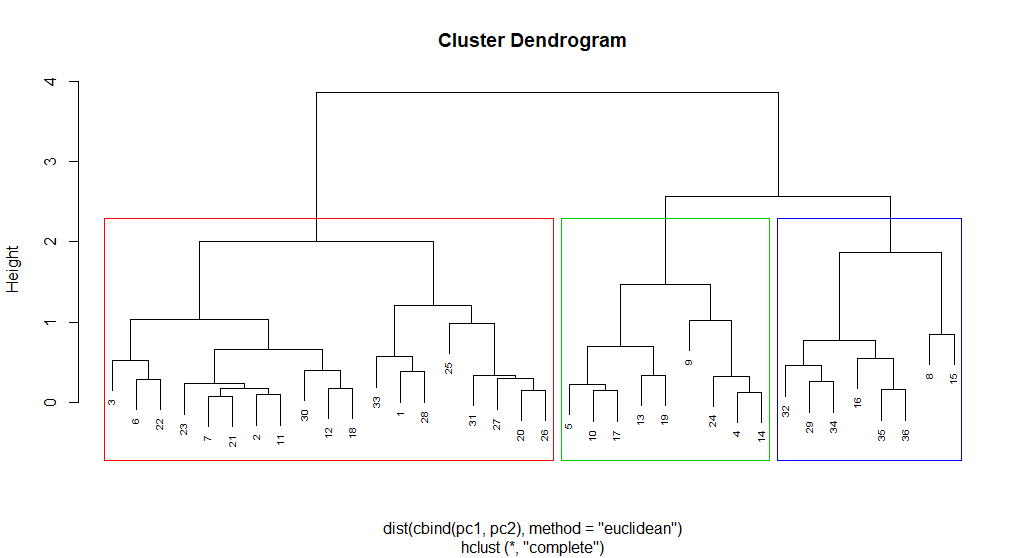
\includegraphics[scale=0.6]{Rplot}
\caption{Hierarchical Clustering with $k=3$}
\label{fig:cluster}
\end{figure}
%%%%%%%%%%%%%%%%%%%%%%%%%%%%%% 
\flushleft{By the 3 clusters we obtain, we can construct its confusion matrix as}
\begin{center}
\begin{tabular}{ c|c c c|c } 
 \# observations & Method 1 & Method 2 & Method 3 & Total \\ \hline
 Cluster 1 & 7 & 5 & 7 & 19\\
 Cluster 2 & 4 & 5 & 0 & 9 \\
 Cluster 3 & 1 & 2 & 5 & 8\\ \hline
 Total  & 12 & 12 & 12 & 36\\ 
\end{tabular}
\end{center}

\begin{lstlisting}[caption=R code for Q3]
#Q3
X <- ds[3:6]
pc1 <- c(t(ev$vectors[,1])%*%t(X))
pc2 <- c(t(ev$vectors[,2])%*%t(X))

clusters <- hclust(dist(cbind(pc1,pc2),method = "euclidean"))
plot(clusters, cex=0.6)
rect.hclust(clusters, k=3, border=2:4)
clusterCut <- cutree(clusters, 3)
table(clusterCut, ds$method)
\end{lstlisting}

\end{solution}

% --------------------------------------------------------------
% You don't have to mess with anything below this line.
% --------------------------------------------------------------
 
\end{document}